\documentclass{article}
\usepackage{amsmath, amssymb}
\usepackage{listings}
\usepackage{enumerate}
\usepackage{bm}
\usepackage{fullpage}
\usepackage{empheq}
\usepackage{graphicx}
\usepackage{caption}
\usepackage{subcaption}
\usepackage{todonotes}

\title{CS 267 Parallel Computing Homework 2\\
\large{Part I (Serial \& OpenMP)}}
\author{Chiyu ``Max" Jiang, Eleanor Cawthon, Madeleine Traverse}
\usepackage[utf8]{inputenc}
\usepackage{color}

\definecolor{mygreen}{rgb}{0,0.6,0}
\definecolor{mygray}{rgb}{0.5,0.5,0.5}
\definecolor{mymauve}{rgb}{0.58,0,0.82}

\lstset{ %
  backgroundcolor=\color{white},   % choose the background color; you must add
                                   % \usepackage{color} or \usepackage{xcolor}
  basicstyle=\ttfamily,        % the size of the fonts that are used for the code
  breakatwhitespace=false,         % sets if automatic breaks should only happen
                                   % at whitespace
  breaklines=true,                 % sets automatic line breaking
  captionpos=b,                    % sets the caption-position to bottom
  commentstyle=\color{mygreen},    % comment style
  deletekeywords={...},            % if you want to delete keywords from the
                                   % given language
  escapeinside={\%*}{*)},          % if you want to add LaTeX within your code
  extendedchars=true,              % lets you use non-ASCII characters; for
                                   % 8-bits encodings only, does not work with
                                   % UTF-8
  frame=single,	                   % adds a frame around the code
  keepspaces=true,                 % keeps spaces in text, useful for keeping
                                   % indentation of code (possibly needs
                                   % columns=flexible)
  keywordstyle=\color{blue},       % keyword style
  language=Python,                 % the language of the code
  otherkeywords={*,...},           % if you want to add more keywords to the set
  numbers=left,                    % where to put the line-numbers; possible
                                   % values are (none, left, right)
  numbersep=5pt,                   % how far the line-numbers are from the code
  numberstyle=\tiny\color{mygray}, % the style that is used for the line-numbers
  rulecolor=\color{black},         % if not set, the frame-color may be changed
                                   % on line-breaks within not-black text (e.g.
                                   % comments (green here))
  showspaces=false,                % show spaces everywhere adding particular
                                   % underscores; it overrides 'showstringspaces'
  showstringspaces=false,          % underline spaces within strings only
  showtabs=false,                  % show tabs within strings adding particular
                                   % underscores
  stepnumber=2,                    % the step between two line-numbers. If it's
                                   % 1, each line will be numbered
  stringstyle=\color{mymauve},     % string literal style
  tabsize=2,	                   % sets default tabsize to 2 spaces
  title=\lstname                   % show the filename of files included with
                                   % \lstinputlisting; also try caption instead
                                   % of title
}
\newcommand{\defeq}{\overset{\text{def}}{=}}
\begin{document}
\maketitle
\section{Introduction}
The primary objective of this project is to implement an $\mathcal{O}(n)$
complexity algorithm to simulate particle dynamics solely dependent on
short-range forces, and extend the serial implementation to a shared-memory
and a distributed memory implementation. We begin in
Section~\ref{section:impl} by describing our changes to the provided
implementations, and analyzing their theoretical and experimental complexity. We
then examine analyze the performance of our code using VTune in
Section~\ref{section:vtune}, and discuss potential further improvements.  We
conclude with an evaluation of the scalability of our two parallel approaches in
Section~\ref{section:scale}.
\section{Implementation Notes and Complexity}\label{section:impl}
\subsection{Getting Serial to $\mathcal{O}(n)$}\label{subection:serial}
Before parllelizing our code, we first needed to improve the reference serial
implementation from which we would build our parallel versions and to which we
would be comparing them. We implemented two different improved serial
algorithms.
\subsubsection{Barnes-Hut Tree}
The first algorithm we implemented utilizes a data-structure which is
called a Barnes-Hut Tree \cite{barnes1986hierarchical}.
Barnes-Hut Tree algorithm is essentially an order $\mathcal{O}(n\log n)$
algorithm. However since this algorithm is more generally extensible to particle
simulations that take into consideration the long-range force interaction and
provides an efficient framework for simplifying it, it is still of interest to
implement and compare this data structure with the binning method. The
Barnes-Hut tree data structure is based on the quad tree data structure.
Initializing the data structure involves breaking the simulation domain
into finer and finer quadrants until each quadrant contains at most one
particle. Organized in this way, clusters of particles can be represented by the
center of mass of the cluster. Under certain threshold conditions, this can
be a good enough approximation.  Since the depth of a balanced quad tree is
$\mathcal{O}(\log n)$, the complexity of this algorithm is $\mathcal{O}(n\log
n)$. This is not ideal in terms of efficiency compared to the binning method,
but it is significantly more efficient that the naive implementation which is
order $\mathcal{O}(n^2)$.

\subsubsection{Binning Method}
We used a binning method to implement the Serial code. By dividing the space
of the simulation into bins, we were able to do far fewer computations as
compared with the original code. For each particle, the
\texttt{apply\_forces()} function was only applied to the particles in that
particle's bin and in the bins that neighbored it, so for a given particle, the
runtime would be $\mathcal{O}(9b n)$ instead of $\mathcal{O}(n^2)$.
% For our
% code, the slope of the line of best fit in the \todo{Eleanor or Madeleine will
% look up what the graph is that gets us this number to clarify this (This slope
% was an output of the Autograder, the graph is the values tested by the
% autograder, but I'm not sure how to graph it since there are 2 variables:
% number of threads and number of particles)} fit is 1.031.

We accomplished the binning by creating a matrix of C++ vectors, with each
position in the matrix representing a single bin. We recreated this matrix at
the start of each time step to adjust for the movement of the particles (which
may have switched bins). An improvement for the serial code would be to edit the
existing matrix instead of creating a new one, but since creating the matrix is
only an $\mathcal{O}(n)$ operation, we did not think the improvement would be
appreciable.

To find the optimal number of bins for the simulation, we set the minimum size
of the bin to the cutoff/100.  We then used a search to find the optimal bin
size. As shown in Figure~\ref{fig:bin_time}, we found 16 bins to be optimal for
reducing simulation time.

\begin{figure}[ht]
\centering
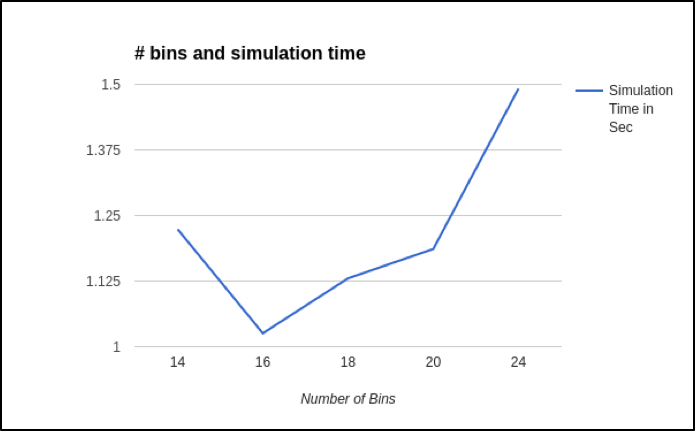
\includegraphics[width=0.7\textwidth]{Picture1.png}
\caption{Plot of number of bins vs. simulation time in the serial simulation.
  This plot indicates that optimal performance is achieved when the number of
  bins is set to 16.}
\label{fig:bin_time}
\end{figure}

\subsubsection{Complexity test}
It is apparent from the small error margins with respect to the log-log linear
best fit lines in Figure~\ref{fig:serial} that both functions run in polynomial
time, that is, $\mathcal{O}(n^k)$ for some constant $k$.  Interestingly,
although Barnes-Hut's theoretical runtime is $\mathcal{O}(n\log n)$ rather than
$\mathcal{O}(n)$, empirically for the values we tested, we found that Barnes-Hut
conformed more closely to the idealized $\mathcal{O}(n)$ performance.

The autograder's calculation of the slope of the best fit curves differs
slightly from that shown in Figure~\ref{fig:serial}: While our graph simply
does a linear regression on the entire set of data, the autograder computes an
average of piecewise slopes. This has the effect of reducing the impact of
degraded performance with large numbers of particles, as the piecewise slope
estimates indicate our binning code achieves much closer to $\mathcal{O}(n)$ at
lower values of $n$, with slopes ranging from 0.598 to 2.381 for an average
slope of 1.570 $\pm$ 0.892. While $\mathcal{O}(n^{1.570})$ is a significant
improvement over the original $\mathcal{O}(n^2)$, it is also significantly
slower than our hoped-for $\mathcal{O}(n)$. We believe this is due to
inefficiences in our implementation (discussed further in
Section~\ref{section:vtune}) rather than to a problem with our algorithm.

In contrast, although Barnes-Hut performs worse in absolute terms for most
tested values of $n$, it scales much more consistently, with an overall slope of
1.260 in our graph and 1.270 as computed by the autograder from a range of
slopes varying just $\pm$ 0.07. This suggests that the low density of our
simulation allows the $n$ term to dominate the $\log(n)$ term in the Barnes-Hut
theoretical runtime --- in other words, our tree is shallow.

% It can be observed that with binning method, the overall average slope for
% log-log plot is lower (1.1409), however the it shows an increasing trend in log
% time for greater $n$. Barnes-Hut tree based algorithms shows more consistent
% polynomial order performance regardless of $n$.
%
\begin{figure}[ht!]
\centering
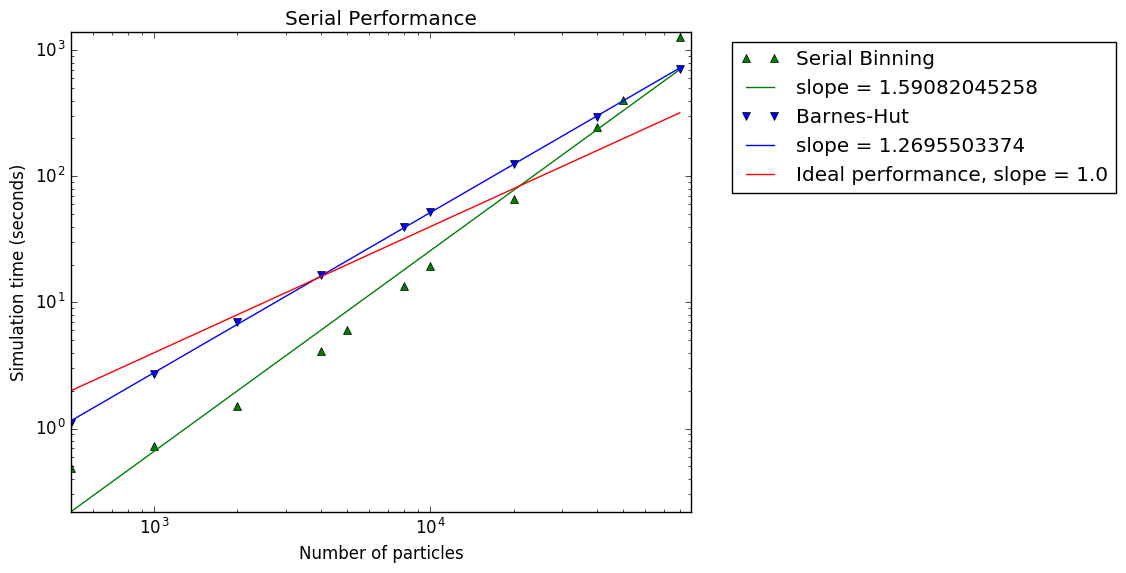
\includegraphics[width=0.9\textwidth]{serial.png}
\caption[Serial complexity plot]{log-log plot of number of particles versus
  simulation time for performance analysis on the two serial methods. Note: The
  ``Ideal performance'' line is meant to illustrate the ideal slope. The
  y-intercept was chosen for visual clarity and is not analytically
  significant.}\label{fig:serial}
\end{figure}
% \begin{figure}[h!]
% \centering
% 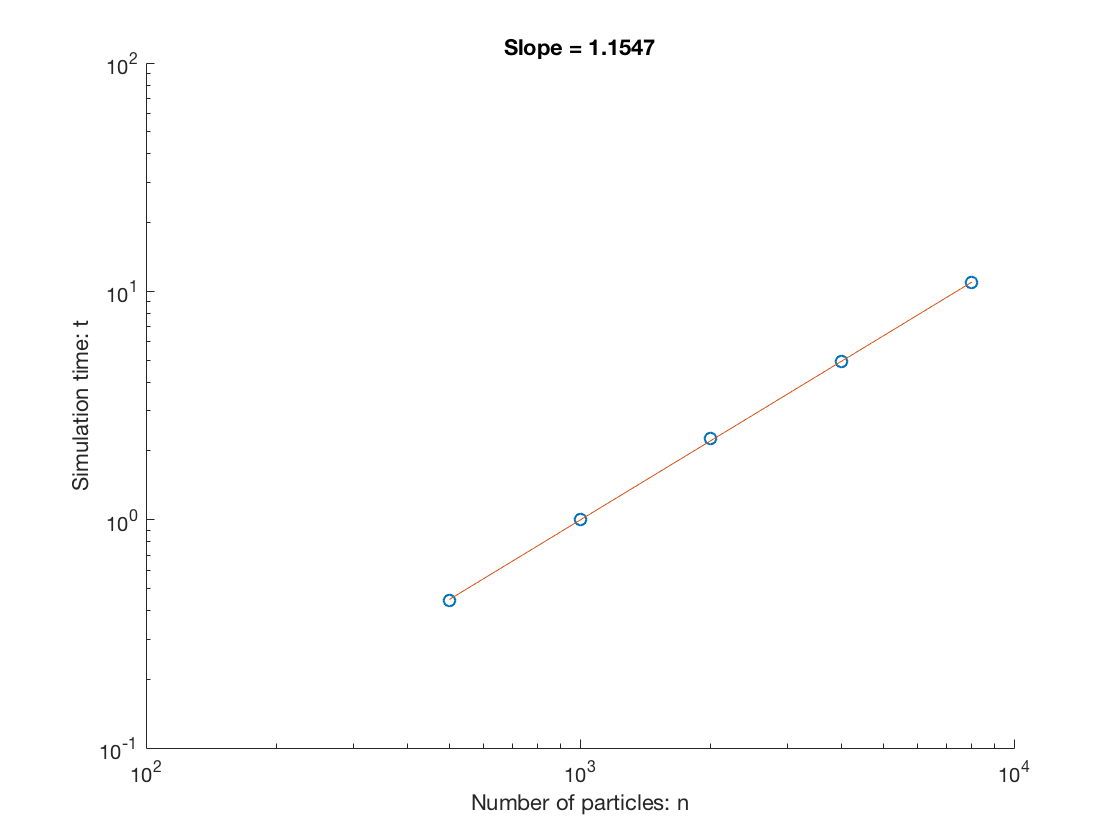
\includegraphics[width=0.7\textwidth]{Picture5.png}
% \caption{log-log plot of number of particles versus simulation time for
% performance analysis on Barnes-Hut method code.}\label{fig:loglogBH}
% \end{figure}
%

\subsection{Shared Memory Implementation with OpenMP}
\label{subsection:openmp}
\subsubsection{Binning Method}
To create the OpenMP code, the serial code with binning was reorganized to allow
for OpenMP Pragmas. The comparing of the particles in the bin matrix was
parallelized by collapsing the matrix for loops into one long process that could
be divided between threads. The scheduler was set to dynamic, however no
statistically significant difference was observed between static and dynamic
allocation. We also attempted to parallelize the creation of the bin matrix at
the beginning of the timestep, but constant segfaults suggested that the code
was not compatible with the pragmas used as the threads were attempting to
create infinite bins.
\subsubsection{Barnes-Hut Tree}
In our first serial implementation of the Barnes-Hut Tree approach, we
re-created the entire particle tree every time the simulation moved to a new
step. Although this did not affect the Big-O runtime, this involved double the
amount of work per step, which is significant even though it is a constant
factor. It also made the code difficult to parallelize because the initial
construction of the tree requires synchronization, introducing a serialized
bottleneck. For these reasons, we decided it was important to enable our
implementation to make updates to the already-constructed tree, allowing
sub-trees to be updated in parallel. Unfortunately, implementing this
functionality proved substantially more difficult than expected, and we
ultimately abandoned this variant due to time constraints. As such, we did not
parallelize the Barnes-Hut variant.

\subsection{Distributed Memory Implementation with MPI}
We explored two basic approaches to converting our binning algorithm to use
distributed memory. We conceptualized our algorithm as requiring two basic
steps: dividing the particles into bins, and distributing particles to the
processors. As such, we had a choice between having the master thread divide
particles into bins and then sending a bin and its neighbors to each process, or
to first distribute particles to processors and then have each process perform
the binning on its subset of the particles. Our preliminary results led us to
adopt the second approach, based on a combination of expected programmer
efficiency and compute efficiency.

% In more detail, our implementation follows the following steps:
% \begin{enumerate}
%   \item The
% \end{enumerate}

\section{Performance Analysis}\label{section:vtune}
\subsection{Serial}
The serial code used the binning method to allow for fewer particle comparisons.
This was very successful. In the Naive code, \texttt{apply\_force} took 1.60e12.
In our code, it took 4.83e10 clock ticks. This is clearly a significant
improvement.

According to the VTune report, the serial code was mostly Back-End bound, taking
up around 31\% of the performance time. This can often be due to data-cache
misses or stalls. Of the Back-End use, \~28\% was Core bound. This metric is
sometimes due to dependencies in program data. Further analysis of the code
breakdown pinpointed the slow down as an issue with the dynamically allocated
vectors used in the matrix map. The performance problem with creating the
vectors is primarily an issue due to the way C++ creates vectors. A small amount
of space is malloced and then, whenever the vector exceeds that space, another
larger space is malloced and everything in the first space must be copied into
the second. Since this was happening multiple times for each time step, the
performance was negatively affected. The choice of the pointer particles to be
stored as vectors was made to allow the matrix to be edited each time-step
instead of requiring it to be rebuilt. The time to build the matrix, however,
was $\mathcal{O}(n)$ time, and is in fact probably mostly negligible, so a far
better storage for the particles would be an array.

The serial code performance could also be improved by using a quadtree structure
for the bins instead of a simple matrix. Even fewer \texttt{apply\_force}
function would need to be called, which would reduce the overall runtime.
\subsection{OpenMP}
The openMP code used the binning method in serial, but distributed the bins to
different threads. In the Naive code for an n of size 12,000,
\texttt{apply\_force} took 1.33e12 clock ticks. Our code for the same n took
3.24e8 clock ticks, a significant improvement.

According to the VTune report, the code was heavily Back-End bound, taking up
around 70\% of the time. Of the Back-End time, \~43\% was Memory Bound. When
this metric is high, it can be due to stalls waiting for memory loads and
stores. This was again discovered to be a consequence of using the dynamically
allocated vectors and could be fixed by using arrays. Other improvements relate
to improving the serial version of the code, as mentioned with the quad tree
bins.
\subsection{MPI}
The MPI code was designed to take advantage of the relatively low latency
involved in communication between nodes. This allows for memory to be
distributed, which can be important with very large data sets. Consequently, the
largest performance cost is in this communication. According to the Craypat
Profile, the \texttt{MPI\_Alltoallv} call takes up between 19-21\% of the
sampling and performance time. The other three MPI calls combined take up \~10\%
of the performance time. A solution to decrease the time spent on the
\texttt{MPI\_Alltoallv} would be to require one processor to hold all of the
data, instead of distributing it.  This “master” would then only send the
required bins to each processor and they would not need to communicated with
each other. If the data is too large not to distribute it, a more complex model
with multiple “masters” could be implemented where they communicate with each
other to keep the data up-to-date.

The performance slowdown of the dynamic vectors from the original serial code is
present in the MPI implementation as well and could be fixed by switching the
data structure to arrays.

A strong benefit was seen again in the MPI code versus Naive due to the binning.
Where the Naive code spent \~67\% of the performance time on
\texttt{apply\_force}, our code spent only \~37\%, a major improvement. This is
due to the fact that binning greatly cuts down on the number of times the
function needs to be called. It could be reduced even further by implementing a
quad-tree structure for the bins so that less particles need to be compared.
\section{Results At Scale}\label{section:scale}
Perhaps due to inherited inefficiencies in our serial code, we encountered
difficulty in scaling to the target $n = 50,000$ particles per processor. We
include data from the only tests that terminated at this scale: our serial
codes, our OpenMP code with 50,000 particles per processor at one and two
processors, and all strong scaling trials with our OpenMP code. Our MPI code at
this scale did not terminate within the allotted time. Accordingly, we also
tested with $n = 5,000$ for strong scaling and $n = 5,000 \times p$ for weak
scaling to $p$ processors.
\subsection{Serial vs. OpenMP vs. MPI: Weak Scaling}
In Figure~\ref{fig:weak}, we compare the execution time of each parallel run to
the execution time for our binning code to run a given number of
particles-per-processor on a single processor. Steeper (more negative) slopes
correspond to more degraded performance with increased $n$, and therefore worse
scalability. The y-axis shows a scalar between 0 and 1, where 1 would represent
perfect scaling where $p$ processors can simulate $n \times p$ particles in the
same time it takes one processor to simulate $n$ particles.

The line with slope = 0 is the theoretical ideal performance with perfect
parallelism. However, calling this performance ideal is misleading, as it does
not take into account Amdahl's Law. A more representative comparison is the
comparison of the slopes of the two serial methods with the slopes of the
parallel methods. The two serial methods have the same slope as exhibited in
Figure~\ref{fig:serial}, but negative.\footnote{The numbers are slightly
  different because only results with $n \ge 4000$ are included in
  Figure~\ref{fig:weak}, whereas Figure~\ref{fig:serial} includes results
with smaller $n$, on which our binning algorithm performs better.}

At similar scale ($4000 < n < 120000$), both OpenMP and MPI exhibit similar
scalability, with slopes very close to $-1$. This means that for both
parallel implementations, each time the number of processors is
doubled, the extent of the speedup is halved. Our limited results for $n=50,000$
show that at least for for OpenMP, the amount of overhead per particle
per processor continues to increase as the problem size grows. The best fit line
for MPI fits the data more closely, suggesting more consistent overhead in that
implementation. However, the absolute performance of MPI is substantially worse
than that of OpenMP.

We note that the performance of OpenMP with one thread is almost identical to
the performance of our serial code. This speaks to the usability of OpenMP as a
library --- it was relatively easy to write code that, without modification,
reduces to the serial runtime without incurring overhead from the
additional code required for OpenMP.
\begin{figure}[ht!]
\centering
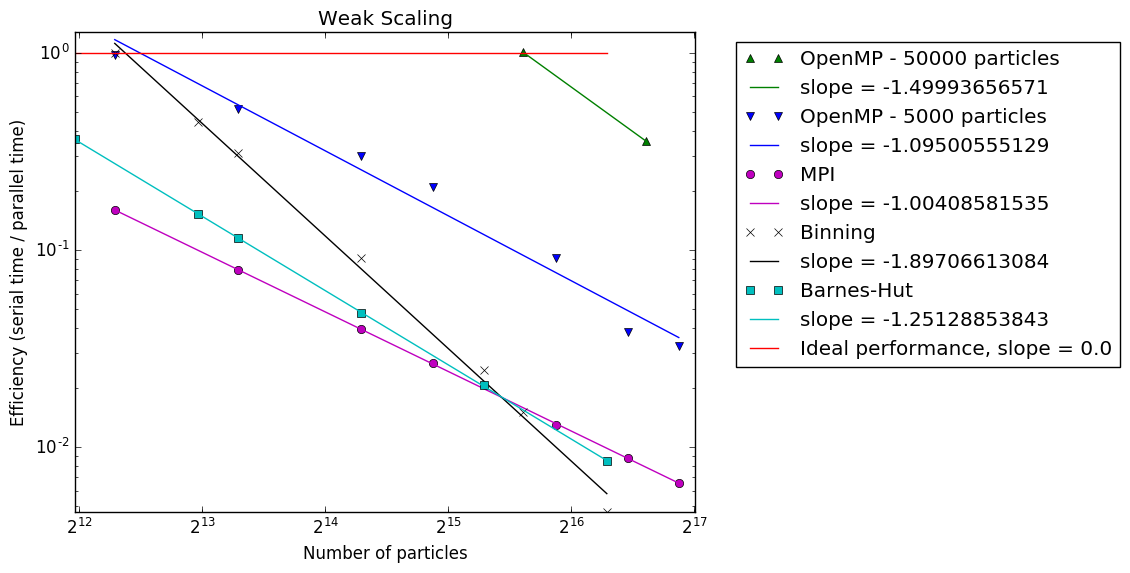
\includegraphics[width=0.9\textwidth]{weak.png}
\caption{Weak scaling results, OpenMP vs. MPI vs. Binning vs.
Barnes-Hut. OpenMP particle numbers are per processor. MPI was tested
with 5,000 particles per processor. The two serial methods were tested
on a single processor with varying numbers of particles.}\label{fig:weak}
\end{figure}

\subsection{OpenMP vs. MPI: Strong Scaling}
In Figure~\ref{fig:strong}, we vary the number of processors while keeping $n$
constant. In this graph, the slope represents the amount of speedup per
processor, with ideal speedup represented by a slope of -1.0 corresponding to
runtime of time $T/p$, where $T$ is the runtime on a single processor.

In our OpenMP code with $n=5000$, the overhead of adding processors obviates the
performance gains at $p > 12$. The data is very close to linear (in log-log
scale) for $p \le 12$. For larger problems, however, our OpenMP code continues
to scale well for all $p$ tested, as demonstrated by the series with $n=50,000$.

As with weak scaling, the absolute performance of our OpenMP code is
significantly better than that of our MPI code for equivalent problems. We
attribute this to the increased complexity of debugging and profiling
distributed memory as compared with shared memory.
\begin{figure}[ht!]
\centering
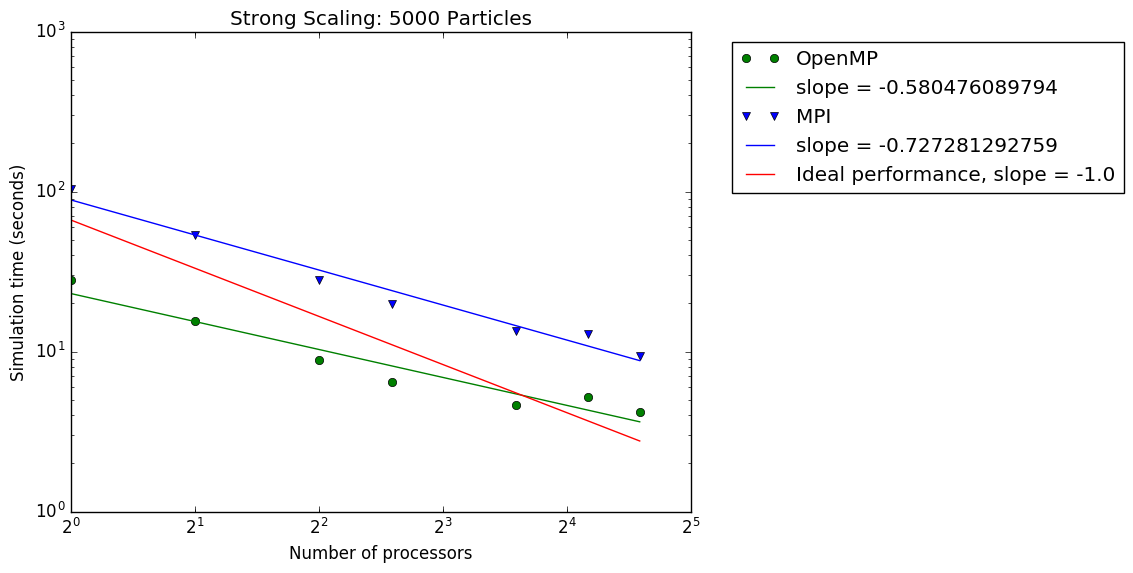
\includegraphics[width=0.9\textwidth]{strong.png}
\caption{Strong scaling results, OpenMP vs. MPI. The y-intercept of
the ideal performance line is the average of three runs of our binning
code with 5000 particles.}\label{fig:strong}
\end{figure}
% \subsection{Overhead of }
% Serial outperforms OpenMP in numbers of particles less than 2000. This makes
% sense because the overhead needed for thread creation in OpenMP cannot be
% ameliorated by the overall decrease in simulation time Figure~\ref{fig:smol}
% illustrates this crossover point at an appropriate scale. However, once the
% number of particles is more than 2000, OpenMP does vastly better, as exhibited
% on the log-log plot in Figure~\ref{fig:strong}. Serial
% struggles with more particles in an accelerated rate, while OpenMP threads
% manage the increase in particles with a linear increase.
% \begin{figure}[h]
% \centering
% 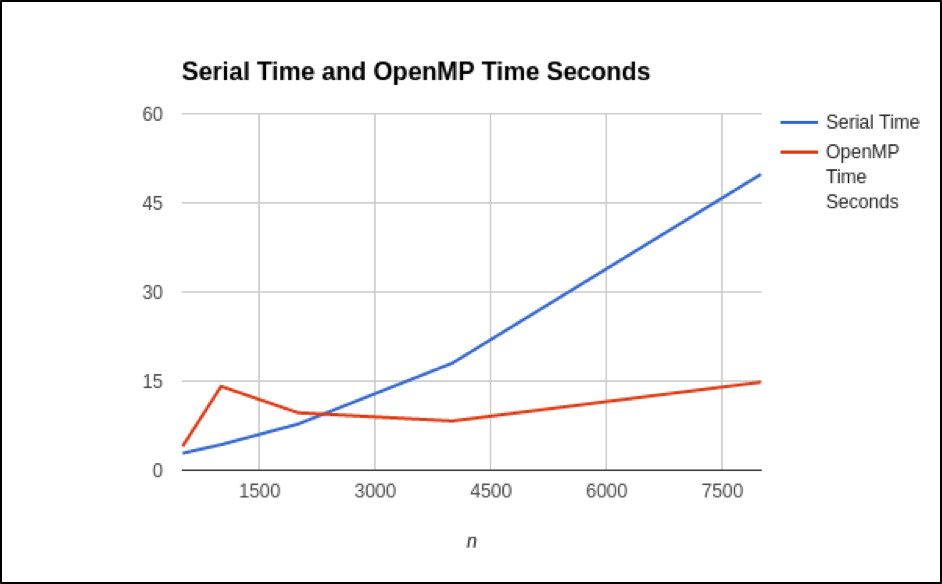
\includegraphics[width=0.7\textwidth]{Picture3.png}
% \caption{Comparison between serial time and OpenMP implementations for low
%   values of $n$. $x$ axis shows particle density and $y$ axis shows running
% time.}\label{fig:smol}
% \end{figure}
\clearpage
\bibliography{main.bib}
\bibliographystyle{unsrt}

\end{document}

